% scRareRefine Bioinformatics-style draft v2.
% Compile from paper/: latexmk -pdf scRareRefine_bioinformatics_draft_v2.tex
\documentclass[11pt]{article}

\usepackage[utf8]{inputenc}
\usepackage[T1]{fontenc}
\usepackage{times}
\usepackage[margin=1in]{geometry}
\usepackage{amsmath,amssymb}
\usepackage{graphicx}
\usepackage{booktabs}
\usepackage{array}
\usepackage{caption}
\usepackage[numbers,sort&compress]{natbib}
\usepackage[hidelinks]{hyperref}

\graphicspath{{figures/}{../results/comparison/}}
\captionsetup{font=small,labelfont=bf}

\newcommand{\method}{scRareRefine}
\newcommand{\rare}{r}
\newcommand{\rts}{\texttt{rare\_train\_size}}

\title{\bfseries \method: risk-controlled rescue of low-frequency cell types under rare-label scarcity}
\author{[Author names]\\[2pt]
\small [Affiliations]\\
\small Correspondence: [email]}
\date{}

\begin{document}
\maketitle

\noindent\textbf{Manuscript category:} Gene expression \\
\textbf{Article type:} Original Paper \\
\textbf{Running title:} Risk-controlled rare-cell rescue

\section*{Structured Abstract}

\noindent\textbf{Motivation:}
Semi-supervised single-cell annotation models can miss low-frequency cell
types when only a small number of rare-class labels are available. A useful
refinement method should recover these missed cells without creating a broad
false rare-cell call set.

\noindent\textbf{Results:}
We introduce \method, a post-hoc refinement module for scANVI that combines
train-derived latent prototypes with validation-only conformal calibration.
\method\ targets a pre-specified low-frequency class and abstains when
validation evidence does not support rescue. Across eight human and mouse
scRNA-seq datasets, nine methods, four rare-label budgets and three seeds, the
scarce-label settings contained only 0.0206\%--0.3526\% labeled rare cells in
training. In these settings, \method\ achieved mean rare-cell F1 of 0.801,
compared with 0.646 for scANVI and 0.665 for kNN, and was best or tied-best in
23 of 24 dataset-budget cells. Its maximum false rare-call rate was 0.009878
under a pre-specified 0.01 budget.

\noindent\textbf{Availability and Implementation:}
Source code, configuration files, and result-generation scripts will be
released at [GitHub URL] and archived at [Zenodo DOI]. The implementation is in
Python using scvi-tools, Scanpy and AnnData.

\noindent\textbf{Contact:} [email]

\noindent\textbf{Supplementary information:}
Supplementary data are available at [URL].

\section{Introduction}

Single-cell RNA sequencing has made it routine to profile complex tissues at
cellular resolution, but the cell types that are most biologically interesting
are often not the most abundant. Rare immune subsets, endocrine subtypes,
tissue-resident stromal cells and lineage intermediates may account for only a
few percent of a dataset. They are also the classes for which labels are most
fragile: small reference panels contain few positive examples, batch-heldout
evaluation can place the target class in different technical contexts, and
semi-supervised classifiers may collapse an under-represented class into a
nearby majority class.

This creates a practical failure mode for cell-type annotation. A model can
achieve acceptable global accuracy while systematically losing the cell type
under study. The problem is not simply that the class is rare in the full
dataset. For a supervised or semi-supervised annotation model, the more direct
quantity is the fraction of training cells that are labeled examples of the
target rare class. In the experiments below, every formal target rare class has
dataset-level prevalence below 5\%, but the scarce-label regimes are more
severe: after downsampling rare labels in the training split, labeled rare
cells comprise only 0.0206\%--0.3526\% of all training cells in the main
scarce-label settings.

Existing annotation methods approach the problem from different directions.
scANVI learns a semi-supervised latent representation and classifier from
labeled and unlabeled cells \citep{lopez2018scvi,xu2021scanvi}. CellTypist,
TOSICA and related supervised systems provide scalable annotation using
marker-informed or transformer-based models \citep{dominguez2022celltypist,chen2023tosica}.
Rebalancing and rare-cell detection methods, including scBalance and scCAD, are
designed to counter class imbalance or discover unusual populations.
Prototype-based approaches such as ProtoCloud use geometric summaries of
reference labels. These methods are valuable, but they do not directly address
a specific deployment question: when a known low-frequency target class is
missed by a semi-supervised classifier, can we selectively recover likely false
negatives while controlling false rare-cell calls?

\method\ is designed for this setting. It is not a de novo rare-cell discovery
method and it does not change the scANVI training objective. Instead, it is an
inductive post-hoc module applied after scANVI. It builds latent-space
prototypes from labeled training cells, scores candidate cells by their
proximity to the target rare prototype relative to other class prototypes, and
uses validation cells to decide whether rescue is needed and how permissive the
rescue rule should be. The final relabeling threshold is calibrated from
validation non-rare cells under a fixed false rare-call budget. If the target
class is not geometrically separable, if the baseline already recovers the
validation rare cells, or if no candidate rank satisfies the validation safety
criterion, the method abstains and returns the baseline predictions.

We evaluate \method\ against eight baselines or alternative methods across
eight datasets covering human and mouse samples, multiple tissues, three random
seeds and four rare-label budgets. The benchmark includes six human datasets
and two mouse Tabula Muris Senis 10x add-on datasets, enabling cross-tissue and
cross-species breadth while preserving within-dataset train-validation-test
evaluation. The main claim is that \method\ recovers rare-cell annotations
under rare-label scarcity with a pre-specified false rare-call budget, and that
it abstains when rescue is not warranted.

\section{Materials and Methods}

\subsection{Problem setup}

Let a single-cell dataset contain gene-expression matrix $X$, cell-type labels
$y$ for a subset of cells, and a pre-specified target rare class $\rare$. The
target class is supplied by the dataset configuration rather than inferred
automatically from a frequency threshold. We use the full labeled dataset only
to define the evaluation target and then construct inductive train, validation
and test splits. Model fitting, prototype estimation, rank selection and
threshold calibration use only training and validation information. Test labels
are reserved for final evaluation.

We distinguish two notions of rarity. The first is the dataset-level target
prevalence,
\[
  \pi_\rare = N_\rare / N,
\]
where $N_\rare$ is the number of cells of the configured target rare class and
$N$ is the dataset size. This is the biological and benchmarking definition
used to select target classes. In the formal benchmark, after excluding the
exploratory \texttt{tabula\_lung\_stroma} dataset, all configured target rare
classes have $\pi_\rare < 5\%$.

The second is rare-label availability in the training split,
\[
  \lambda_\rare = L_{\rare,\mathrm{train}} / N_{\mathrm{train}},
\]
where $L_{\rare,\mathrm{train}}$ is the number of labeled rare-class training
cells retained after rare-label downsampling and $N_{\mathrm{train}}$ is the
total number of training cells. This is the operational scarcity seen by the
classifier. The label budgets \rts{} $=0.01, 0.05, 0.10$ retain approximately
1\%, 5\% or 10\% of training rare labels, with a minimum of five labeled rare
cells when available; \rts{} $=$ \texttt{all} retains all training rare labels.
Across the formal eight-dataset benchmark and three seeds, the scarce-label
settings correspond to $\lambda_\rare = 0.0206\%$--$0.3526\%$ of training
cells.

\subsection{Data splitting and label masking}

The primary experiments use batch-heldout splits. Cells are partitioned into
training, validation and test sets by batch when dataset metadata supports this
design, with fallback logic handled by the preprocessing pipeline. Because
batches have unequal sizes, the resulting split proportions need not exactly
match nominal ratios, but the split is fixed before model fitting and is
recorded in the run manifest. This design tests whether a rare-cell recovery
rule transfers across held-out experimental batches rather than only across
randomly sampled cells.

Within the training split, rare-class labels are downsampled according to the
selected label budget. Non-rare labeled cells remain available, while rare
cells whose labels are masked are treated as unlabeled for semi-supervised
training. Validation and test labels are not downsampled for evaluation;
validation labels are used only for method selection and calibration, and test
labels are used only for final metrics.

\subsection{scANVI backbone and prototype scoring}

The backbone model is scANVI, trained through scvi-tools on highly variable
genes selected within the pipeline. The model first learns a latent
representation with scVI and then fits the semi-supervised scANVI classifier
using labeled and unlabeled training cells. For each split, the pipeline exports
predicted labels, class probabilities and latent embeddings. These exported
embeddings are shared by \method\ and by comparison scripts where applicable,
with manifest checks to prevent accidental reuse across incompatible
configurations, splits or datasets.

\method\ builds class prototypes in the scANVI latent space using labeled
training cells. For each class $c$, the prototype $\mu_c$ is the mean latent
vector of labeled training cells of class $c$. A class-specific radius $\rho_c$
is estimated from within-class distances to the prototype, using the median
distance with a conservative fallback for extremely small classes. Distances
from a cell embedding $z_i$ to each prototype are normalized by these radii.

The rare-membership score is computed from normalized prototype distances so
that cells closer to the target rare prototype, relative to competing
prototypes, receive higher scores. We also compute the rank of the rare
prototype among all class prototypes for each cell. A cell is considered a
rescue candidate only if the scANVI prediction is not the target rare class and
the rare prototype rank is at most $k$, where $k$ is selected on validation data
from the grid $\{1,2,3\}$. This candidate rule limits rescue to cells that are
already geometrically close to the rare prototype.

\subsection{Validation-only gates and conformal calibration}

\method\ applies three validation-only safeguards before relabeling test cells.
First, a separability gate compares the distance between the target rare
prototype and the nearest non-rare prototype against the within-rare radius. If
the target rare class is insufficiently separated, with separability below 1.3,
the method abstains. This constant is treated as a pre-specified conservative
prior rather than tuned per dataset.

Second, a necessity gate checks whether rescue is supported by validation
errors. If the validation split contains too few missed rare cells by the
baseline, or if scANVI already recovers the target rare class on validation,
\method\ abstains. This prevents unnecessary relabeling when the baseline is
already saturated or when validation evidence is too sparse to select a
reliable rescue rule.

Third, the method selects the maximum candidate rank $k$ from $\{1,2,3\}$ using
validation performance under a safety constraint. Candidate ranks are evaluated
by validation rare F1 subject to a Wilson upper-bound constraint on false
rare-cell calls. Ties are broken toward the smaller rank, yielding a more
conservative rule.

After a rank is selected, the final rare-score threshold is calibrated from
validation non-rare cells. Let $s_i$ be the rare-membership score for validation
cells whose true label is not $\rare$. The threshold is a finite-sample high
quantile corresponding to a pre-specified false rare-call budget $\alpha=0.01$
\citep{vovk2005algorithmic,angelopoulos2023conformal}. At test time, a non-rare
scANVI prediction is changed to the target rare class only if the cell passes
the selected rank rule and its rare-membership score exceeds the calibrated
threshold. Otherwise, the original scANVI prediction is retained.

\subsection{Datasets, methods and metrics}

The formal benchmark contains eight datasets. Six are human datasets spanning
immune, pancreas, lung, stomach and small intestine contexts. Two mouse Tabula
Muris Senis 10x datasets were added to broaden the evaluation across species
and tissues. The configured target rare classes are fixed in dataset
configuration files and are not selected post hoc from model performance.

\begin{table}[t]
\centering
\caption{Formal benchmark datasets and target rare classes.}
\label{tab:datasets}
\small
\begin{tabular}{lll}
\toprule
Configuration & Context & Target rare class \\
\midrule
\texttt{immune\_dc} & human immune atlas & ASDC \\
\texttt{pancreas\_baron} & human pancreas & gamma / epsilon \\
\texttt{pancreas\_integrated} & integrated human pancreas & endothelial \\
\texttt{tabula\_lung\_endo} & human lung & endothelial subtype \\
\texttt{tabula\_sapiens\_stomach} & human stomach & mast cell \\
\texttt{tabula\_small\_intestine} & human small intestine & intestinal tuft cell \\
\texttt{mouse\_lung\_tms\_10x} & mouse lung, TMS 10x & vein endothelial cell \\
\texttt{mouse\_pancreas\_tms\_10x} & mouse pancreas, TMS 10x & pancreatic D cell \\
\bottomrule
\end{tabular}
\end{table}

We compare \method\ with scANVI, kNN on the shared latent representation,
CellTypist, scBalance, ProtoCloud, HiCat, scCAD and TOSICA. All methods are
evaluated on the same dataset splits, seeds and rare-label budgets where
applicable. The complete comparison grid contains eight datasets, four label
budgets, three seeds and nine methods, for 864 runs. The final result table
contains 864 successful runs.

The primary metric is rare-class F1 on the independent test split. We also
report rare-class precision and recall, because the method is intended to
recover rare false negatives rather than only improve aggregate annotation
accuracy. The safety metric is the false rare-call rate among true non-rare
cells, reported in the result files as \texttt{rare\_fp\_rate}. The scarce-label
region is defined as \rts{} in $\{0.01,0.05,0.10\}$.

\section{Results}

\subsection{Rare-label scarcity is more severe than target-class prevalence}

All formal target classes are low-frequency classes in their respective
datasets, with full-dataset prevalence below 5\%. However, the label-scarcity
experiment is governed by the number of labeled rare cells available to the
training process. In the most stringent settings, the classifier sees only a
handful of rare labels against thousands of non-rare training cells. For
example, in \texttt{immune\_dc} at \rts{} $=0.01$, the training split contains
277 rare cells and 11,014 non-rare cells, but only five rare cells remain
labeled, giving $\lambda_\rare = 5/(277+11014)=0.0443\%$.

This framing clarifies the evaluation target. The task is not to discover an
arbitrary cluster below a fixed frequency threshold. The task is to preserve
and recover a known low-frequency class when labeled positive examples are
scarce enough that a semi-supervised classifier may erase the class from its
predictions.

\subsection{\method\ improves rare-cell F1 in scarce-label settings}

In the scarce-label region, \method\ achieved the highest mean rare-cell F1
across methods. Averaged over datasets, seeds and scarce-label budgets, its
rare-cell F1 was 0.8008, compared with 0.6645 for kNN and 0.6463 for scANVI.
The improvement is driven by recall recovery: \method\ mean rare recall was
0.7543, compared with 0.5883 for kNN and 0.5855 for scANVI.

\begin{table}[t]
\centering
\caption{Mean performance in scarce-label settings. Max false rare-call rate is the maximum over scarce-label runs.}
\label{tab:scarce}
\small
\begin{tabular}{lrrrr}
\toprule
Method & Rare F1 & Recall & Mean FP rate & Max FP rate \\
\midrule
\method & 0.8008 & 0.7543 & 0.0012 & 0.0098 \\
kNN & 0.6645 & 0.5883 & 0.0002 & 0.0035 \\
scANVI & 0.6463 & 0.5855 & 0.0003 & 0.0023 \\
scBalance & 0.5827 & 0.4967 & 0.0001 & 0.0021 \\
ProtoCloud & 0.5592 & 0.4776 & 0.0002 & 0.0018 \\
CellTypist & 0.5514 & 0.4688 & 0.0002 & 0.0012 \\
scCAD & 0.4726 & 0.6698 & 0.0246 & 0.0752 \\
TOSICA & 0.4345 & 0.3918 & 0.0030 & 0.0209 \\
HiCat & 0.1445 & 0.1193 & 0.0000 & 0.0002 \\
\bottomrule
\end{tabular}
\end{table}

The method was also robust at the dataset-budget level. Collapsing over seeds
gives 24 scarce-label dataset-budget cells. \method\ was exactly best or
tied-best in 23 of 24 cells. In the only non-best cell,
\texttt{tabula\_small\_intestine} at \rts{} $=0.10$, ProtoCloud achieved rare
F1 of 0.9848 and \method\ achieved 0.9823, a difference of 0.0025.

\begin{figure}[t]
\centering
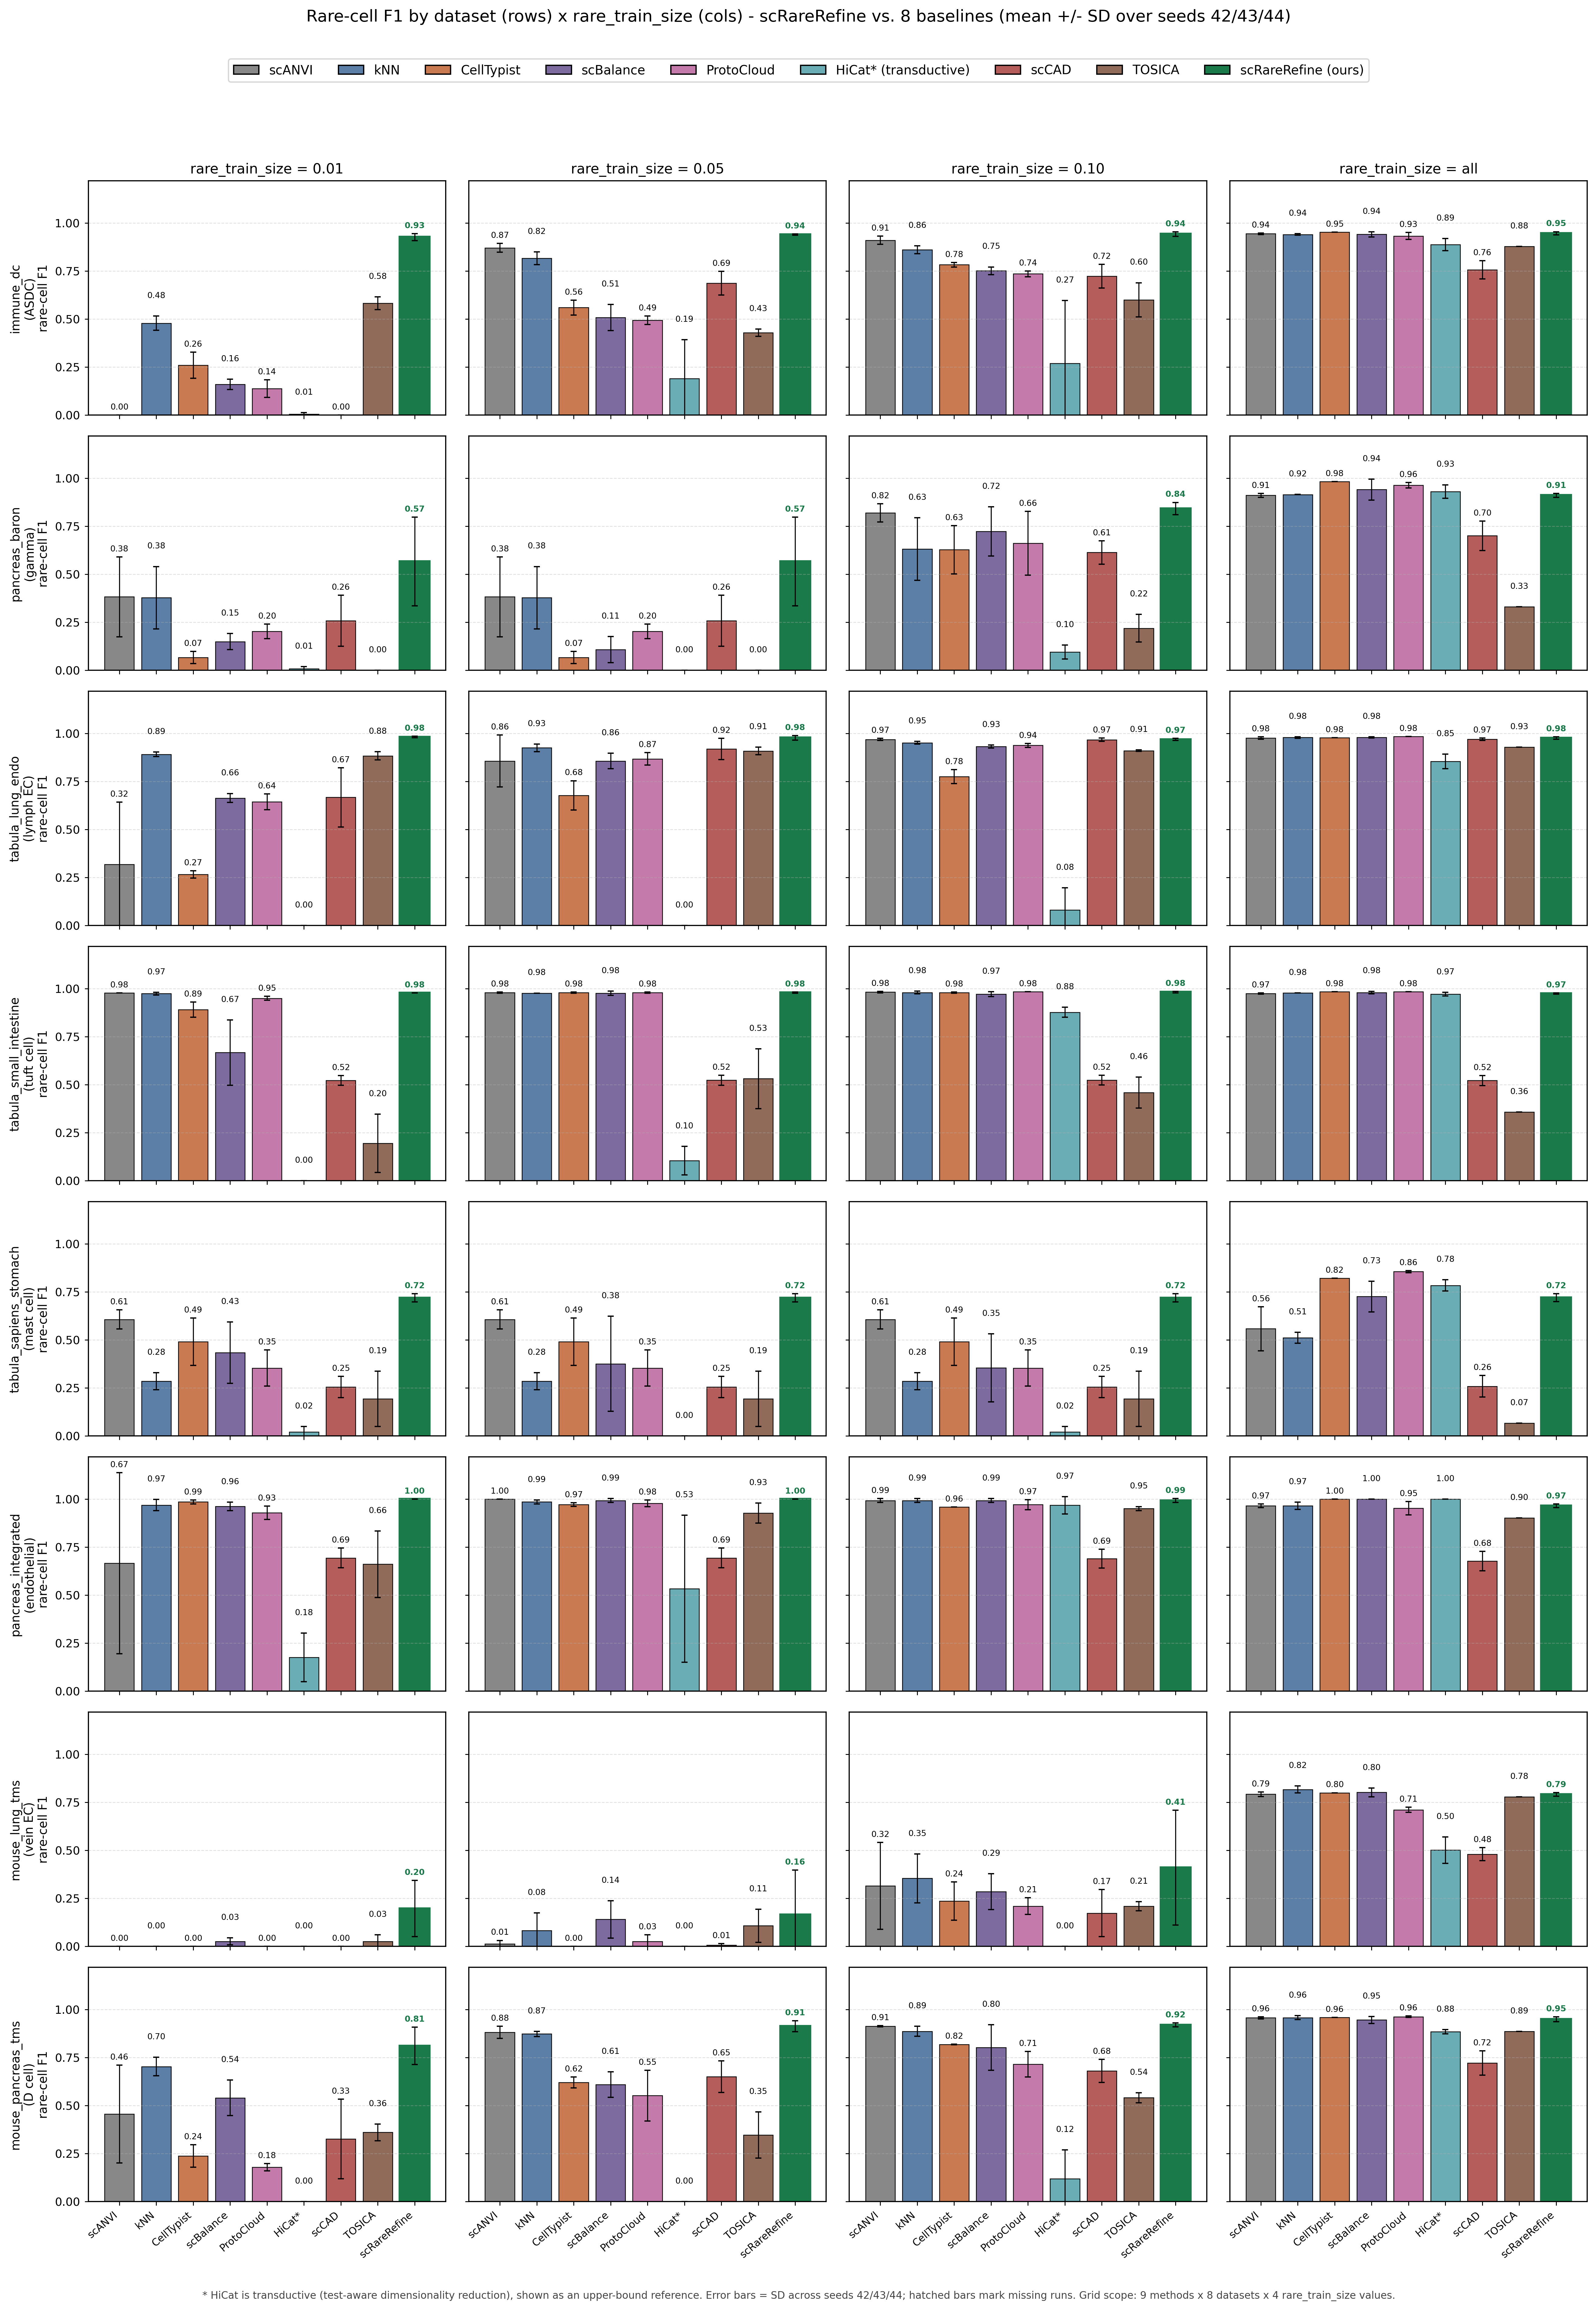
\includegraphics[width=0.88\linewidth,height=0.68\textheight,keepaspectratio]{comparison_bars_grid.png}
\caption{Eight-dataset comparison grid generated from the current comparison summary. The full result table contains 864 successful runs across eight datasets, four rare-label budgets, three seeds and nine methods.}
\label{fig:grid}
\end{figure}

\subsection{Paired comparisons show consistent gains}

We compared \method\ against each method in matched dataset-budget-seed units in
the scarce-label region ($n=72$ paired units per baseline). Against scANVI,
\method\ had 41 wins, 30 ties and one loss, with mean paired $\Delta$F1 of
+0.1545 and bootstrap confidence interval [+0.0956,+0.2199] (one-sided paired
Wilcoxon $P=8.82\times10^{-9}$). The large number of ties is expected: if
validation evidence indicates that rescue is unnecessary or unsafe, \method\
returns the baseline prediction.

\begin{table}[t]
\centering
\caption{Paired scarce-label rare-F1 comparisons. Differences are paired by dataset, rare-label budget and seed.}
\label{tab:paired}
\small
\begin{tabular}{lrrrrr}
\toprule
Comparator & Win & Tie & Loss & Mean $\Delta$F1 & 95\% CI \\
\midrule
scANVI & 41 & 30 & 1 & +0.1545 & [+0.0956,+0.2199] \\
kNN & 59 & 8 & 5 & +0.1363 & [+0.0967,+0.1773] \\
CellTypist & 65 & 4 & 3 & +0.2494 & [+0.1950,+0.3049] \\
scBalance & 61 & 5 & 6 & +0.2181 & [+0.1642,+0.2737] \\
ProtoCloud & 62 & 6 & 4 & +0.2416 & [+0.1884,+0.2972] \\
HiCat & 66 & 5 & 1 & +0.6563 & [+0.5795,+0.7291] \\
scCAD & 66 & 5 & 1 & +0.3282 & [+0.2815,+0.3771] \\
TOSICA & 67 & 2 & 3 & +0.3663 & [+0.3064,+0.4261] \\
\bottomrule
\end{tabular}
\end{table}

Because paired units are correlated across seeds and some rare-label budgets
collapse to the same effective label count, these $P$ values should be read as
directional evidence alongside effect sizes and confidence intervals, not as
strictly independent-sample tests.

\subsection{False rare-cell calls remain within the pre-specified budget}

Recovering more rare cells is only useful if the rare label remains specific.
Across the complete eight-dataset comparison, including the \texttt{all}
label-budget setting, the maximum false rare-call rate observed for \method\
was 0.009878, below the pre-specified $\alpha=0.01$ budget. This maximum
occurred in \texttt{mouse\_lung\_tms\_10x} at \rts{} $=$ \texttt{all} for one
seed. In the scarce-label region, the largest values remained close to, but
below, the same budget.

The comparison methods show different safety profiles. Some methods, such as
kNN and scANVI, have low false rare-call rates but miss many rare cells. Others,
such as scCAD in this benchmark, recover more rare cells but can exceed the
false rare-call budget. \method\ occupies the intended middle ground: it
increases rare recall relative to scANVI while using validation calibration to
constrain broad rare-label expansion.

\subsection{Cross-tissue and mouse add-on datasets support broader applicability}

The original human benchmark covers multiple tissue contexts, including immune,
pancreas, lung, stomach and small intestine datasets. The two mouse Tabula Muris
Senis 10x add-on datasets extend this breadth to a second species and
additional tissue contexts while keeping the same evaluation contract. These
mouse datasets are not treated as a separate domain-transfer experiment in
which a model is trained on human cells and tested on mouse cells. Rather, they
test whether the same label-scarcity and rescue procedure remains useful
outside the original human-only panel.

The inclusion of mouse lung and mouse pancreas reduces the risk that the method
is tuned to a single organism or tissue geometry. The main aggregate results
include these two datasets, and the complete 864-run comparison succeeded
without method-specific changes to the \method\ algorithm.

\section{Discussion}

The central result is that a constrained post-hoc rescue module can recover
rare-cell annotations lost by a semi-supervised backbone under severe label
scarcity. \method\ improves rare-cell F1 and recall across an eight-dataset
benchmark while keeping the observed false rare-call rate below a fixed 1\%
budget. The method is deliberately narrow: it targets one configured
low-frequency class, builds prototypes only from labeled training cells,
calibrates thresholds only on validation cells, and abstains when validation
evidence is insufficient.

This narrowness is a practical advantage. Many single-cell studies do not need
a fully new annotation model; they need to know whether a small, known cell type
has been erased by the combination of class imbalance and batch shift. Because
\method\ operates after scANVI, it can be attached to an established
semi-supervised workflow and audited through its gates, candidate ranks and
calibrated threshold. When it changes predictions, the change is traceable to
latent prototype proximity and validation-calibrated rare-score evidence. When
it does not change predictions, the abstention is also informative.

The evaluation highlights why rare-cell benchmarking should report both target
prevalence and labeled rare-cell availability. A target class below 5\% is
biologically low-frequency, but the model's difficulty depends on how many
labeled rare examples remain in the training set. Reporting $\lambda_\rare$
makes clear that the method is being tested under a true rare-label regime,
rather than simply on datasets containing low-frequency classes.

There are several limitations. First, \method\ assumes the target rare class is
known in advance. It is therefore complementary to de novo rare-cell discovery
methods rather than a replacement for them. Second, the current implementation
refines a single target rare class per run. Multi-rare-class settings may
require class-wise calibration or a joint error-budget allocation. Third, the
method inherits the quality of the scANVI latent representation. If rare and
majority cells are not separable in the latent space, the conservative gates
will abstain or recall will remain bounded. Fourth, while the benchmark now
includes mouse add-on datasets, it does not test direct human-to-mouse model
transfer. Finally, the current manuscript reports computational results from
public scRNA-seq datasets; experimental validation of newly recovered rare
cells would require independent biological assays or marker-level confirmation.

\section{Conclusion}

\method\ provides a validation-calibrated post-hoc rescue procedure for known
low-frequency cell types in scRNA-seq annotation. By combining train-only
latent prototypes, validation-selected candidate ranks, conformal score
thresholds and abstention gates, it improves rare-cell recovery under severe
rare-label scarcity while maintaining a fixed false rare-call budget. The
current eight-dataset benchmark supports \method\ as a practical refinement
module for studies where preserving a known rare cell type is more important
than maximizing aggregate annotation accuracy.

\section*{Data availability}

All datasets used in this study are derived from public single-cell resources,
including human atlas datasets and CELLxGENE/Tabula Muris Senis mouse 10x
subsets. Processed dataset identifiers, download instructions and preprocessing
scripts will be provided in the repository and Supplementary Data. No new
sequencing data were generated for this study.

\section*{Code availability}

The \method\ implementation, configuration files, comparison scripts, plotting
scripts and result manifests will be made freely available at [GitHub URL]
under [license]. The submitted version will be archived at [Zenodo DOI].
Reproducibility instructions will include the two conda environments used for
the comparison grid: \texttt{scanvi311} for the scANVI/\method\ pipeline and
most baselines, and \texttt{sandbox310} for baselines requiring older dependency
stacks.

\section*{Funding}

This work was supported by [funding information].

\section*{Conflict of Interest}

The authors declare no competing interests.

\section*{Acknowledgements}

The authors thank the maintainers of scvi-tools, Scanpy, AnnData, CELLxGENE,
Tabula Sapiens and Tabula Muris Senis for public data and software resources.

\section*{Internal author notes, not for submission}

This is an AI-assisted working draft for author rewriting. Bioinformatics
follows the ISCB policy on large language models; before submission, the
manuscript must be substantially revised by the authors, all references and
numerical claims must be checked against final artifacts, and AI assistance
must be disclosed where required.

Open items before submission: verify every reference and DOI; decide whether
ablation results should be rerun on all eight datasets or clearly labeled as
six-human ablation; add final GitHub and Zenodo URLs; convert to the official
Bioinformatics or BMC Bioinformatics template after the scientific content is
frozen.

\begin{thebibliography}{99}

\bibitem[Lopez et~al.(2018)]{lopez2018scvi}
Lopez, R., Regier, J., Cole, M.B., Jordan, M.I. and Yosef, N. (2018)
Deep generative modeling for single-cell transcriptomics.
\emph{Nature Methods}, 15, 1053--1058.

\bibitem[Xu et~al.(2021)]{xu2021scanvi}
Xu, C., Lopez, R., Mehlman, E., Regier, J., Jordan, M.I. and Yosef, N. (2021)
Probabilistic harmonization and annotation of single-cell transcriptomics data
with deep generative models. \emph{Molecular Systems Biology}, 17, e9620.

\bibitem[Dominguez Conde et~al.(2022)]{dominguez2022celltypist}
Dominguez Conde, C., Xu, C., Jarvis, L.B. et~al. (2022)
Cross-tissue immune cell analysis reveals tissue-specific features in humans.
\emph{Science}, 376, eabl5197.

\bibitem[Chen et~al.(2023)]{chen2023tosica}
Chen, J., Xu, H., Tao, W., Chen, Z., Zhao, Y. and Han, J.-D.J. (2023)
Transformer for one stop interpretable cell type annotation.
\emph{Nature Communications}, 14, 223.

\bibitem[Vovk et~al.(2005)]{vovk2005algorithmic}
Vovk, V., Gammerman, A. and Shafer, G. (2005)
\emph{Algorithmic Learning in a Random World}. Springer.

\bibitem[Angelopoulos and Bates(2023)]{angelopoulos2023conformal}
Angelopoulos, A.N. and Bates, S. (2023)
Conformal prediction: a gentle introduction.
\emph{Foundations and Trends in Machine Learning}, 16, 494--591.

\bibitem[Tabula Sapiens Consortium(2022)]{tabulasapiens2022}
The Tabula Sapiens Consortium. (2022)
The Tabula Sapiens: a multiple-organ, single-cell transcriptomic atlas of
humans. \emph{Science}, 376, eabl4896.

\bibitem[Tabula Muris Consortium(2018)]{tabulamuris2018}
Tabula Muris Consortium. (2018)
Single-cell transcriptomics of 20 mouse organs creates a Tabula Muris.
\emph{Nature}, 562, 367--372.

\bibitem[Tabula Muris Senis Consortium(2020)]{tabulamurissenis2020}
Tabula Muris Senis Consortium. (2020)
A single-cell transcriptomic atlas characterizes ageing tissues in the mouse.
\emph{Nature}, 583, 590--595.

\bibitem[Baron et~al.(2016)]{baron2016pancreas}
Baron, M., Veres, A., Wolock, S.L. et~al. (2016)
A single-cell transcriptomic map of the human and mouse pancreas reveals
inter- and intra-cell population structure. \emph{Cell Systems}, 3, 346--360.

\end{thebibliography}

\end{document}
